\documentclass[dvipdfmx]{jsarticle}
\usepackage[T1]{fontenc}
\usepackage[dvipdfmx]{hyperref}
\usepackage{lmodern}
\usepackage{latexsym}
\usepackage{amsfonts}
\usepackage{amssymb}
\usepackage{mathtools}
\usepackage{nccmath}
\usepackage{amsthm}
\usepackage{multirow}
\usepackage{graphicx}
\usepackage{wrapfig}
\usepackage{here}
\usepackage{float}
\usepackage{ascmac}
\usepackage{url}

\title{クラスタリング・分類・相関ルール分析に関する調査}
\author{文理学部情報科学科\\5419045 高林 秀}
\date{\today}

\begin{document}

\maketitle

\begin{abstract}
本稿は、今年度データ科学2のレポート課題として、「クラスタリング」、「分類(決定木)」および「相関ルール分析」の各分野に関して、各手法の特徴やアルゴリズムの説明、解説を行うものである。また、1年次に学習したlatexを使用したpdf作成の復習も兼ねるものである。
\end{abstract}

\section{目的}
本稿は、今年度データ科学2の最終レポート課題として「クラスタリング」、「分類(決定木)」および「相関ルール分析」の各分野に関して、各手法の特徴やアルゴリズムの説明、数式等の解説を行うものである。それぞれの分野の各手法の特徴やアルゴリズムに言及した上、使われている数式の解説を記載する。
\section{基礎導入}
\subsection{データマイニングとは}
まず、本稿で取り扱う分野の大元であるデータマイニングについて軽く説明する。データマイニングとはビックデータや企業の顧客情報など大量のデータが格納されたデータベースから機械学習や、統計計算等の手法でデータを分析し、そこから新たに有用な知識を発見しようという技術である。データマイニングでは、データから得られる情報を分析しそこから得ることのできる知識を取り出すことである。つまり、そこから先の得た知識をどう利用するかは人間の判断に委ねられている。すなわち、データマイニングで行うのは知識の発掘であり、発掘した知識が有用か、またどう活用するかは人間が判断する、ということだ。\par
大きく分けてデータマイニングは以下のように分類することができる。
\begin{enumerate}
  \item 仮説検証的データマイニング
  \begin{enumerate}
    \item 推定
    \item 分類
  \end{enumerate}
  \item 知識探索的データマイニング
  \begin{enumerate}
    \item 相関ルール分析(アソシエーションルール分析)
    \item クラスタリング
  \end{enumerate}
\end{enumerate}
上記の分類はあくまで大別であり、実際は手法により当てはまる分野は異なる。\par
仮説検証的データマイニングは、仮説に沿ってある課題を解決するためにデータ分析を行うことを示す。機械学習の手法のみならず従来までの統計的手法が使用されることも多い。\par
知識探索的データマイニングは、データベース上のデータから特定のルールや規則、パターンといった知識を探索するためにデータ分析を行うことを示す。こちらは機械学習やディープラーニング等の手法が多く用いられる。本稿で扱うのは、上記に示した「分類」、「クラスタリング」、「相関ルール分析」の3つである。
\subsection{機械学習について}
機械学習とは、コンピュータがある問題とその答えを使用して学習を行い、データに潜むパターン等を識別、発見する技術である。この機械学習は大きく3つに系統が別れている。初めに「教師あり学習」、次に「教師なし学習」、最後に「強化学習」である。そしてそこから更に、求める結果や手法によって「分類」「回帰」「クラスタリング」「次元削減」「Q-Learning」と細かく分割される。
\begin{figure}[H]
  \centering
  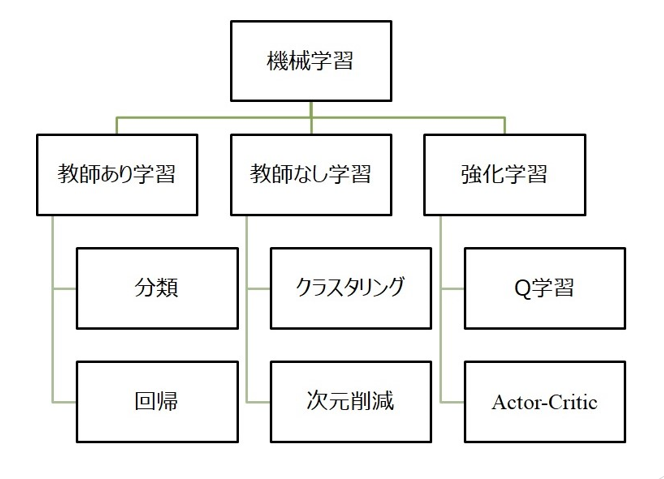
\includegraphics[scale=0.4]{images/ML.PNG}
  \caption{機械学習の枠組み}
\end{figure}
今回説明する、分類は上記分類の「教師あり学習」に、クラスタリングは「教師なし学習」に該当する。教師あり学習と教師なし学習についての具体的な説明は本稿では省略するが、以下にその件に関して記載したレポートのURLを添付する。
\begin{itemize}
  \item 機械学習に関する説明をした過去のレポート:\url{https://drive.google.com/file/d/1wyoRO20UmgiYsxAjkFKLzxhwPvv-xhbx/view?usp=sharing}
\end{itemize}
\section{クラスタリング}
クラスタリングとは、データのグループ分けを行うことをいい、クラスタリングの結果で生じた各データ集合をクラスタと呼ぶ。このクラスタには同じ様な性質をもったデータが集められている。前章で示したとおりクラスタリングは与えられたデータから計算によって自動的にデータの分類、グルーピングを行うので、機械学習では教師なし学習に分類される。\par
クラスタリングは、知識探索的な手法であるので得られた結果は何らかの基準にしたがってクラスタが形成されている。よって、客観的な証拠としてクラスタリングを用いるのは適切ではなく、データの要約など知識や知見を得るために使用するのが適切である。\par
なお、今後の説明で登場するクラスタ内距離やクラスタ間距離などの用語については、今回の課題の説明範囲外なので以下のレポートを参照いただきたい。
\begin{itemize}
  \item クラスタリングの基本に関する説明レポート:\url{https://drive.google.com/file/d/1JP3DnVNmH3kOtEULt73u79zJTb1B1Wvq/view?usp=sharing}
\end{itemize}
クラスタリングは以下に示すように、階層的クラスタリングと非階層的クラスタリングの2つに大別される。
\begin{enumerate}
  \item 非階層的クラスタリング
  \begin{enumerate}
    \item k-平均法(k-means)
  \end{enumerate}
  \item 階層的クラスタリング
  \begin{enumerate}
    \item 凝集型(階層的併合型)
    \item 分岐型
  \end{enumerate}
\end{enumerate}
その他にも、クラスタ間の密度に基づく手法や、格子に基づく手法などに分けることもできるが本稿では省略する。
\subsection{非階層的クラスタリング}
非階層的クラスタリングは、予め分割するクラスタ数$K$を定めたとき、クラスタ内距離を最小にしつつかつクラスタ間距離を最大にするようにクラスタを決定する方法である。このクラスタ数$K$は人間が定めるハイパラメータであり、この$K$の値によってクラスタリング結果は大きく変化する可能性がある。このクラスタ数$K$を自動的に決定する手法はいくつか考案されているが、本稿での説明は省略する。\par
以下は、非階層的クラスタリングの流れの概要である。
\begin{enumerate}
  \item クラスタ数$K$を定める。
  \item データを$k$分割する。
  \item なにかの基準や手法を用いてデータ分割が改善するように、データ分割を繰り返す。
  \item 3の結果、改善される度合いが小さくなればクラスタリング終了。
\end{enumerate}
非階層的クラスタリングの長所として、計算量の少なさが挙げられるだろう。これは後述する手法からも分かるとおり、予め分割するクラスタ数$K$にしたがってデータを分けていく。したがって、階層的クラスタリングよりも計算量が小さくなるという利点がある。よって、データ量が大きい場合(例:ビックデータ分析)のデータ分析に適した手法とされている。\par
反対に、短所として「初期値依存性」が挙げられるだろう。これは、クラスタリングを行う際、最初に$K$個の初期中心点を選択する必要があり、この初期中心点の選択によってクラスタリング結果が大きく変化するという問題である。
\begin{figure}[H]
  \centering
  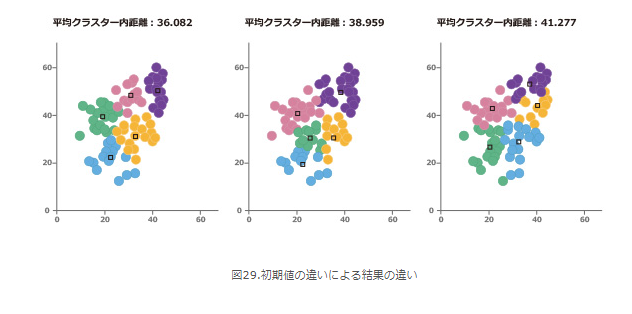
\includegraphics[scale=0.4]{images/k-problem.png}
  \caption{非階層的クラスタリングの初期値依存性の例}
  出典:\url{https://www.albert2005.co.jp/knowledge/data_mining/cluster/non-hierarchical_clustering}
\end{figure}
よって、非階層的クラスタリングを行う際には何回かクラスタリングを実行し、平均クラスタ内距離が最小となる初期中心点を選択する必要が生じる。\par
次は非階層的クラスタリングの代表的手法であるk-平均法(k-means)について説明する。
\subsubsection{k-平均法(k-means)}
k-平均法では以下の目的関数を利用する。この目的関数を最小化するようにデータの分割を行いクラスタを形成していく手法である。
\begin{gather*}
  \Sigma_{k=1}^{K}\Sigma_{x_{i}\in C_{k}}(x_{i}-c_{k})^{2}
\end{gather*}
k-平均法のアルゴリズムは以下に示すとおりである。
\begin{enumerate}
  \item クラスタ数$K$定める。
  \item ある手法に基づいてデータ集合を$K$個のクラスタに分割し、その結果を$C_{n}$とする
  \item 2の結果を$C_{pre}$として保持しておく\par
  以降は、$C_{n}$と$C_{pre}$が一致するまで繰り返しをする。
  \item 各クラスタの重心を計算し、それを新たなクラスタの中心点とする
  \item 各データと中心点との距離を計算し、最も近い中心点のクラスタへの割当を行う→この結果を$C_{n}$とする:目的関数の値が最小化するようにクラスタを更新する
  \item $C_{n}$と$C_{pre}$が一致した場合はクラスタリングを終了し、そうでない場合はもう一度3を行う。\par
  クラスタリング終了時
  \item $C_{n}$を結果として出力する
\end{enumerate}
k-平均法では、各クラスタの重心とクラスタ内距離の総和の局所最適解\footnote{ある範囲における関数の最小値(極小値)のこと。その関数の真の最小値(極小値)は大域的最適解と呼ばれる。}を求めていく。この局所最適解が収束するまで、クラスタ割当の更新と重心の再計算を行う。\par
なお初期クラスタの形成に関しては次の3通りの手法が挙げられる。
\begin{itemize}
  \item 各データに対して、ランダムに1から$K$個のいずれかのクラスタに割当を行う方法
  \item データ全体からランダムに$K$個のデータを選択し、それぞれ{s1~sK}とする。{s1~sK}以外の各データは、{s1~sK}の中で最も近いsi(s1~sKのうちから1つ)のクラスタに割り当てる方法。
  \item データのある空間からランダムに$K$個の点を生成し選択する。それぞれ{s1~sK}とする。各データは{s1~sK}の中で最も近いsi(s1~sKのうちから1つ)のクラスタに割り当てる方法。
\end{itemize}

\subsection{階層的クラスタリング}
前章の非階層的クラスタリングとは異なり、階層的クラスタリングでは予めクラスタ数$K$を定める必要はない。階層的クラスタリングでは、似た性質を持つデータ同士を1つずつグルーピングしていくようにクラスタを形成する。データを1つ1つ比較ししていき、似ているデータ同士、およびクラスタを新たなクラスタとして併合する。そうすると、最終的に階層構造のようなクラスタが出来上がるので、階層的クラスタリングと呼ばれている。\par
先に示したが、階層的クラスタリングには凝集型と分岐型に大別することができる。
\paragraph{凝集型}
凝集型は階層併合的クラスタリングとも呼ばれ、各データを1つのクラスタとして考え各クラスタをボトムアップに併合することで、新たなクラスタを形成する手法である。手順の概要は下記に示すとおり。
\begin{enumerate}
  \item 各データをそれぞれ1つのクラスタと見なす
  \item クラスタの数が1つになるまで次の操作を繰り返す
  \begin{enumerate}
    \item それぞれクラスタ間で距離を算出する
    \item 最も距離が小さいペア同士を新たなクラスタとして併合する
  \end{enumerate}
\end{enumerate}
図で示すと以下のようになる。左から順番に進行する。
\begin{figure}[H]
 \begin{minipage}{0.5\hsize}
  \begin{center}
   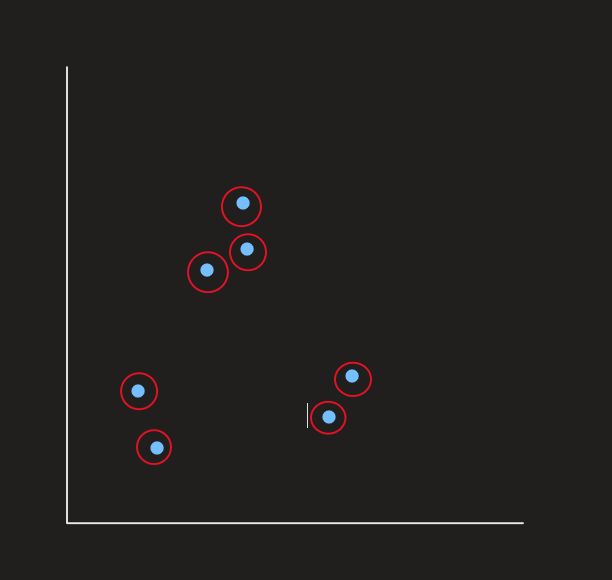
\includegraphics[scale=0.3]{images/gyousyu01.png}
  \end{center}
  \caption{1.各データをそれぞれ1つのクラスタと見なす}
  \label{fig:one}
 \end{minipage}
 \begin{minipage}{0.3\hsize}
  \begin{center}
   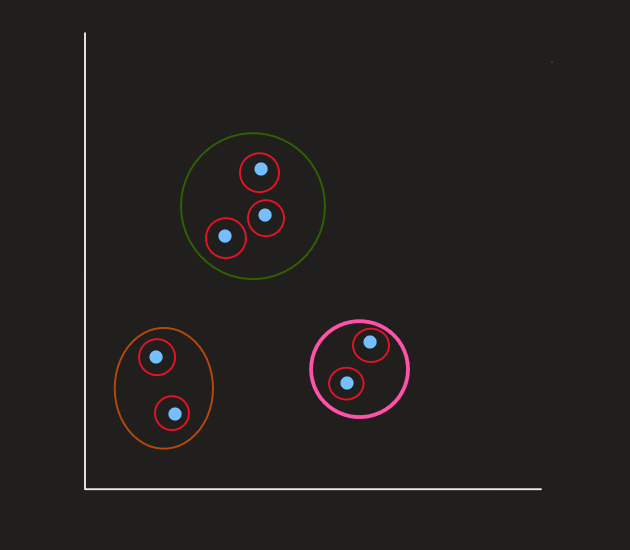
\includegraphics[scale=0.3]{images/gyousyu02.png}
  \end{center}
  \caption{2~(a),(b)クラスタの併合}
  \label{fig:two}
 \end{minipage}
 \begin{minipage}{0.5\hsize}
  \begin{center}
   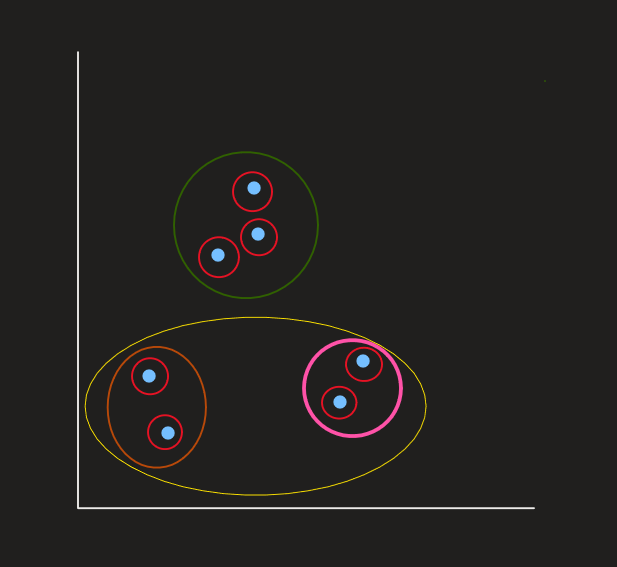
\includegraphics[scale=0.3]{images/gyousyu03.png}
  \end{center}
  \caption{3.クラスタの併合その2}
  \label{fig:two}
 \end{minipage}
 \begin{minipage}{0.5\hsize}
  \begin{center}
   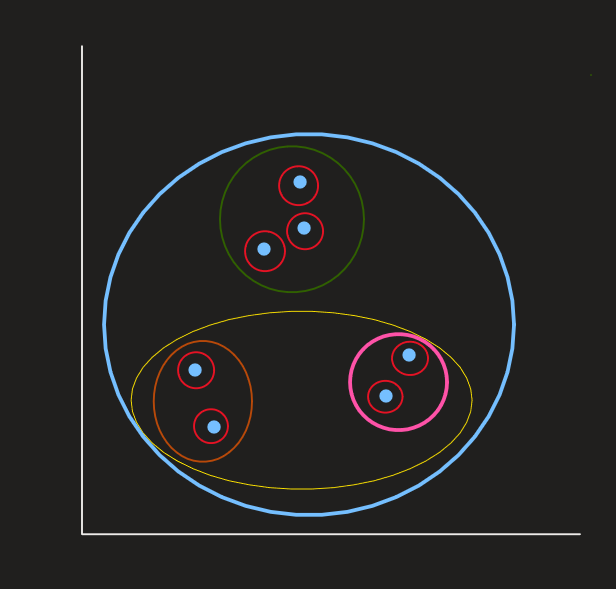
\includegraphics[scale=0.3]{images/gyousyu04.png}
  \end{center}
  \caption{4.クラスタ数が1になったのでクラスタリング終了}
  \label{fig:two}
 \end{minipage}
\end{figure}
より形式的に示す以下の様なアルゴリズムが出来上がる。
\begin{verbatim}
  X:クラスラリング対象のデータ集合
  C := {{x} | x ∈ X}:クラスタの集合C
  while |C| > 1 {
    <C_a, C_b>:=argmin_C_i,C_j ∈ C(D(C_i, C_j))
    C := (C\{C_a, C_b})∪{C_a∪C_b}
  }
\end{verbatim}
凝集型クラスタリングの具体的な計算手法には、利用するクラスタ間距離に応じて下記のものが存在する。
\begin{itemize}
  \item ウォード法(ward法)
  \item 群平均法
  \item 重心法
  \item 最短距離法(単リンク法,単連結法)
  \item 最長距離法(完全リンク法,完全連結法)
  \item 群間平均法
\end{itemize}
\begin{itemize}
  \item $C_{x}$:クラスタの集合
  \item $D(C_{x}, C_{y})$:クラスタ間距離
  \item $M(C_{x})$:クラスタの重心
\end{itemize}
\paragraph{最短距離法}
最短距離法は、異なるクラスタに属している2データ間距離の最小値をクラスタ間距離とする手法である。すなわち、最近点距離である。
\begin{center}
\begin{eqnarray*}
    D(C_{g}, C_{h}) = min_{i \in C_{g}, j \in C_{h}}(dist(i, j)
\end{eqnarray*}
\end{center}
\paragraph{最長距離法}
最長距離法は、異なるクラスタに属している2データ間距離の最大値をクラスタ間距離とする手法である。すなわち、最遠点距離である。
\begin{center}
  \begin{eqnarray*}
    D(C_{g}, C_{h}) = max_{i \in C_{g}, j \in C_{h}}(dist(i, j))
  \end{eqnarray*}
\end{center}
\paragraph{群間平均法}
群間平均法は、異なるクラスタに属している2データ間距離の平均値をクラスタ間距離とする手法である。すなわち、平均距離である。
\begin{center}
  \begin{eqnarray*}
    D(C_{g}, C_{h}) = \frac{1}{|C_{g}|\times |C_{h}|}\Sigma_{i \in C_{g}, j \in C_{h}}dist(i,j)
  \end{eqnarray*}
\end{center}
\paragraph{重心法}
重心法は、各クラスタの重心を求め、その距離をクラスタ間距離とする手法である。すなわち、重心間距離である。
\begin{center}
  \begin{eqnarray*}
    D(C_{g}, C_{h}) = dist(M(C_{g}), M(C_{h}))
  \end{eqnarray*}
\end{center}
\paragraph{ウォード法}
ウォード法は「重心との誤差の改善度合い」に着目し計算する手法である。
\begin{center}
\begin{eqnarray*}
  D(C_{g}, C_{h}) = E(C_{g}\cup C_{h}) - E(C_{g}) - E(C_{h})
  = E(C_{g}\cup C_{h}) - (E(C_{g}) + E(C_{h})) \\
  なお、
  E(C) = \Sigma_{x\in C}dist(x, M(C))^{2} : 重心からの距離の二乗和\\
  ※D(C_{g}, C_{h}):クラスタまたはデータの「併合後の誤差」-「併合前の誤差」
\end{eqnarray*}
\end{center}
\paragraph{分岐型}
凝集型とは異なりトップダウンに各データを分割することでクラスタを形成する。データ集合全体を1つのクラスタと見なし、徐々に小さいクラスタへ分割していく手法である。現在のところあまり使用されていない手法と言える。\par
なお、本稿では分岐型の具体的な説明は省略するが、具体的手法の例として「Diana法」が存在する。\par
\subsection{非階層的クラスタリングと階層的クラスタリングの長所と短所}
前章でも述べたが、非階層的クラスタリングの長所として、計算量の少なさが挙げられるだろう。反対に、短所として「初期値依存性」が挙げられるだろう。\par
階層的クラスタリングの長所として、前章の計算手法で紹介したとおり重心を用いない手法であれば様々な類似度を利用することができる点が挙げられる。加えて、クラスタを併合する際の順番が分かりやすいので、細かくクラスタの変化の様子を追うことができる。これは、階層的クラスタリングの結果として使用する「デンドログラム」の存在が大きな要因になっている。後述する決定木のように、クラスタ併合の課程が樹形図で可視化することができるので、非階層的クラスタリングよりも結果の説明がしやすい。
反対に、欠点としてデータ数が多いと樹形図の把握が困難になり、理解困難になる。また、各事例間に類似度の差が小さい場合、樹形図の鎖状化の発生により、全体的なクラスタを把握するのが難しくなる点がある。その他にも、使用する手法によって様々な問題点を抱えている。以下その一例を示す。
\begin{itemize}
  \item 郡平均法を使用した場合:デンドログラムの反転現象が起こる可能性がある。これはクラスタ間距離の現象により、デンドログラムが交差してしまう現象である。
  \begin{figure}[H]
    \centering
    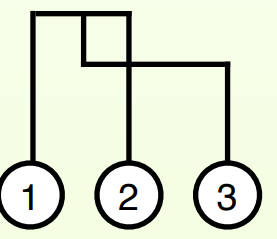
\includegraphics[scale=0.4]{images/dendoroHanten.png}
    \caption{デンドログラムの反転現象の例}
    出典:\url{https://www.kamishima.net/archive/clustering.pdf}
  \end{figure}
  \item 最短距離法:空間濃縮の発生$\Rightarrow$併合後の新クラスタは次の併合の対象となる可能性が加速度的に増加する。
  \item 最長距離法:空間拡張$Rightarrow$併合後の新クラスタは次の併合の対象となる可能性が加速度的に減少する。
\end{itemize}
\section{分類:決定木構築TDIDT}
分類は先に示したとおり、機械学習の教師あり学習に区分される。分類学習では、事前に定められたカテゴリ、およびクラスに入力データを分類することを行う。その一手法として決定木というものが存在する。\par
\subsection{決定木について}
決定木は「木構造を利用した機械学習手法」である。分類を行う決定木を「分類木」、回帰(連続値の予測)を行う決定木は「回帰木」と呼ばれる。決定木では任意の属性の属性値による条件分岐によって、データを徐々に分割することで結果を出力する。したがって、生成される木構造の枝は分割の結果ラベルを、葉は予測、分類されるクラスの結果を、各ノードは属性に関する分割テスト含んでいる。\par
決定木を使用する例として、ミカンとリンゴを分類する場合を考える。下記の図のように、ミカンの画像を4枚、リンゴの画像を2枚の計6枚の画像データセットがあるとする。
これを、ある条件Aを定め、それに当てはまるもの、そうでないものを分割する。この操作を分割テストという。分割テストの結果によって次の分割テスト行うか否かが決定され、最終的に、ミカンとリンゴが図のように分類される。これが決定木の大まかな流れである。
\begin{figure}[H]
  \centering
  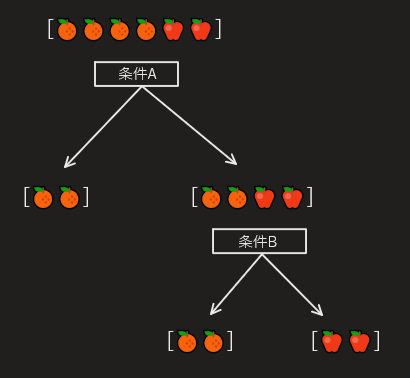
\includegraphics[scale=0.6]{images/decition_ex1.PNG}
  \caption{ミカンとリンゴの分類木}
\end{figure}
以下簡単に決定木の長所、短所をまとめる。
\begin{table}[H]
  \begin{center}
    \caption{決定木のメリット・デメリット}
    \begin{tabular}{|c|c|} \hline
      メリット & デメリット \\ \hline
      ・学習結果の可読性が高く結果の根拠を説明しやすい & ・条件分岐が複雑になるほど過学習しやすい\\
      ・データの前処理が少なく済むことが多い & ・精度が突出して良いわけではない\\
      ・予測時に必要な計算量が小さい & \\
      ・回帰、分類の両方に対応可能 & \\ \hline
    \end{tabular}
    \label{hyo01}
  \end{center}
\end{table}
\subsection{TDIDTについて}
決定木構築手法の代表例として、TDIDT法(Top Down Induction of Decision Trees)がある。この手法は、比較的簡単にコンパクトかつ正確な決定木を作ろうとする概念、すなわちヒューリスティックスに基づいた決定木構築法である。ここでいうTop Downとは、木の根から作るという意味で、Inductionとは、帰納推論、すなわちデータからモデルを構築するという意味である。TDIDTはその属性で分割した後のことは全く考慮していない。つまり、数手先である属性を分割基準にしていればもっと良い決定木ができる、ということを考慮せず、現時点で最良の属性を選択する。したがって貪欲アルゴリズムといわれている。\par
TDIDTの大まかな流れは次の通り。
\begin{enumerate}
  \item 根となるデータ集合を用意する。
  \item ある基準(情報利得・情報利得比・ジニ係数)で属性を選ぶ。
  \item 選ばれた属性の属性値ごとにデータを分割する。
  \item 各枝に対して、3を繰り返す。
  \item 停止条件を満たす場合、その枝の分割を終了とする。
\end{enumerate}
分割属性の選択は、できるだけその属性で分割したときにクラス分布が偏れば、しっかりとデータを分類できるので良い分割基準となる。\par
このとき、分割属性の選択基準として考えられる情報利得・情報利得比・ジニ係数について説明する。なお、本稿では自己情報量等の基本的な数式の説明は省略する。この部分に関しては、以下のリンクから決定木構築のレポートを参照いただきたい。
\begin{itemize}
  \item 決定木構築のレポート:\url{https://drive.google.com/file/d/1QviNpUqGr6yGqpJYqp1gyfWtksf35V6o/view?usp=sharing}
\end{itemize}
\subsubsection{情報利得}
情報利得とは一言で言えば「クラスの偏りがどの程度進んだか」を表す数値である。データセット$D$のおける属性$A$の情報利得の計算式は下記。
\begin{center}
  \begin{align*}
    Gain_{A}(D) = H(D) - H_{A}(D) \\
  \end{align*}
\end{center}
この値が大きいほど、分割テストに適した良い属性ということになる。
$D$を分割する前のエントロピーが$H(D)$で、属性$A$での分割後のエントロピーが$H_{A}(D)$であり、それぞれ下記式で示すことができる。
\begin{center}
  $I(c, D)|c:クラス, D:データセット(データ集合)$とすると、
  \begin{center}
    \begin{align*}
      I(c, D) = -\log_2 P_{D}(c) \\
    \end{align*}
    ※$P_{D}(c)$:$D$中のデータのクラスが$c$となる確率
  \end{center}
  \begin{align*}
    H(D)=\Sigma_{c \in C}P_{D}(c) \times I(c, D)=-\Sigma_{c \in C}P_{D}(c)\log_2 P_{D}(c) \\
  \end{align*}
  \begin{align*}
    H_{A}(D)=\Sigma_{a \in A}p_{D}(a) \times H(D_{a}) \\
  \end{align*}
  $P_{D}(a)$:$D$中のデータの属性$A$の属性値が$a$となる確率。
\end{center}
すなわち、クラス分布を偏らせるためには、情報利得が大きい属性を選択すれば良い。すなわち\textbf{情報利得 = 分割前のエントロピー - 分割後の各エントロピーの重み付き平均}ということになる。\par
しかし、情報利得にはある問題点がある。それは、分割数の大きい属性に対して優先的に高い数値を与えてしまうという点だ。これは、例えば各事例に振られるID番号の例を考えれば分かりやすい。ID番号は事例ごとに1つの数値を割り振っている。したがって、どの属性よりもデータの分割数が大きい属性ということになる。このID属性を分割テストに用いた場合、ある意味完全にデータを分類できるが、ID番号はただの番号、データの順番なので意味をなさない。この様な欠点を補うため、情報利得比と呼ばれる分割基準がある。
\subsubsection{情報利得比}
情報利得比とは、情報利得を分割情報量で正規化した数値である。
\paragraph{分割情報量}分割数が大きい属性に対して、より大きな値をとる性質を持つ。
\begin{center}
  \begin{align*}
    SI_{A}(D) = \Sigma_{a\in A}P_{D}(a) \times I(a, D) = \Sigma_{a\in A}P_{D}(a)\log_2 P_{D}(a)
  \end{align*}
\end{center}
情報利得比$GainRaito_{A}(D)$は下記式で計算される。
\begin{center}
  \begin{align*}
    GainRaito_{A}(D) = \frac{Gain_{A}(D)}{SI_{A}(D)}
  \end{align*}
\end{center}
\subsubsection{ジニ係数(Gini Index)}
分割後のデータ集合の、クラス分布が偏っている時、次の2つのことが言える。
\begin{itemize}
  \item その集合から取り出した2つの事例が同一のクラスに属する確率が高い。
  \item その集合から取り出した2つの事例が同一のクラスでない確率が低い。
\end{itemize}
この状況を利用した属性の評価基準がジニ係数である。ジニ係数では「2つの事例が同一のクラスでない確率」について考える。\par
前にも述べたように、決定木では、同一のクラスに属さない確率が低い方がクラスが偏っていて良いとされる。ここで、属性$A$に対するジニ係数を以下のように定める。
\begin{center}
  \begin{align*}
    Gini_{A}(D) = \Sigma_{a \in A}P_{D}(a) \times G(D_{a}) \\
    G(D) = 1 - \Sigma_{c \in C}P_{D}(c)^{2} \\
    P_{D}(c)^{2}:2事例があるクラスcに属する確率。
  \end{align*}
\end{center}
なお、ジニ係数は、集合から取り出した2つの事例が同一のクラスでない確率が低い、ということを表す数値なので、情報利得とは異なり、\textbf{より小さい値}の属性がよいとされる。\par
5.の停止条件に関して、は以下の場合が該当する。
\begin{enumerate}
  \item すべての事例が同一クラスに属する時 \par
  予測するクラスが1つに定まるので、これ以上データを分割する必要がない。
  \item 分割する属性がない時 \par
  属性が離散属性、すなわちカテゴリである場合、一度分割テストで利用された属性は再度利用することができない。したがって、利用できる属性は徐々に減少していく。分割テストを繰り返す中で、データセットが持ち得る全属性を利用し尽くしてしまった場合、これ以上分割ができない。
  \item 分割の際、条件に合致する事例が少ない時 \par
  分類される事例数がある程度少なくなった場合、そこで分割テストを打ち切る。
  \item 分割に対して良い属性が見つからない時 \par
  すなわち、属性評価において、適切でないと判断された時、その属性で分割してもクラス分布がほとんど変化しないからである。前項でも述べたが、情報利得や情報利得比が小さい時若しくは、ジニ係数が大きい時に起こる。
\end{enumerate}
このTDIDTをC言語での記述を模した疑似コードで表現すると以下のようになる。
※下記で記載している、A\_iやN\_iは数式で表現したときの$A_{i}, N_{i}$に相当する。
\begin{verbatim}
  void generate_decision_tree(N, DS, AL) {
      if(DSに含まれるデータがすべて同一クラスに属する) {
        そのクラスでNのラベル付を行う。
        Nをリーフノード(葉)とする。
        return 0;
      } else if(ALが空である) {
        if(DSの最も標準的なクラスである) {
          Nのラベル付を行う
          Nをリーフノードとする。
        return 0;
        }
      } else {
        最良属性を決定し、その最良属性の値でノードNをラベル付けする。
        for(int i = 0; i < 最良属性の値の種類の個数; i++) {
          最良属性の値A_iの分岐を作成する。
          その分岐を満たすデータ部分集合をS_iとする。
          分岐先のノードをN_iとする。
          if(S_iが空でない) {
            S_iを新たな入力サンプルデータとする。
            ALから最良属性を除いたものを新たな属性リストL_iとする。
            generate_decision_tree(N_i, S_i, L_i);
            決定木を分岐に接続する。
          } else {
            最も一般的なクラスでラベル付されたリーフノードを分岐に接続する。
          }
        }
      }
    }
\end{verbatim}
加えて、TDIDTは分割統治法とも見なされることがある。\par
分割統治法(Divide and conquer)とは、一般に「問題全体をいくつかの小さな問題に分け、各部分の問題を解くことによって計算コスト(計算時間等)を減らそうとする手法」という意味である。\par
TDIDTでは、初めに選択された属性値にしたがってデータ集合をちいさな部分集合に分割する。次に、各部分集合に対して分割テストを行うことで決定木構築を目指す。すなわち、一つの大きな問題「データ集合」を複数の小さな問題「分割後の部分集合」に分けて、処理を進めているので、分割統治法であると言える。\par
決定木構築において、その汎化性能(ロバスト性)を向上させるために、枝刈りが行われることがある。
枝刈りは、過学習している枝、もしくは木を簡略化する手法である。これによって、木そのものが完結になり、分類精度の向上が見込まれる。枝刈りには、大きく分けて事前枝刈りと、事後枝刈りと呼ばれる方法が存在する。
\begin{itemize}
  \item 事前枝刈り\par
  該当する学習例が少ない場合、木の成長を止める手法である。これは、少ないデータに適合させようとすると過学習しやすくなってしまうためで、それを防ぐ目的がある、
  \item 事後枝刈り\par
  木が生成された後に、枝刈りを行う手法。事前枝刈りと比較して、枝刈りによる効果が大きい特徴を持つ。
  \begin{enumerate}
    \item 誤り削減枝刈り
    \item コスト複雑度枝刈り
    \item 悲観的枝刈り
  \end{enumerate}
  などといっいた手法が存在する。
\end{itemize}
\subsubsection{誤り削減枝刈り(reduced-error pruning)}
誤り削減枝刈りとは、決定木に対する誤り削減に基づいた枝刈りアルゴリズムである。\par
入力としては、学習済みの決定木と、検証用データを使用する。このアルゴリズムは枝刈り後の決定木を出力する。
\begin{enumerate}
  \item 決定木の根から遠い順に、木の各ノードに対して以下の操作を行う。
  \begin{enumerate}
    \item そのノード以下の部分木がカバーするデータを分割した際の正解率を計算する:accuraty
    \item そのノード以下の部分木がカバーするデータのマジョリティクラスを計算する:majoriry
    \item もし、accuraty $\leq$majoriryならば、その部分木をマジョリティクラスの葉に置き換える。
  \end{enumerate}
  \item 枝刈り後の決定木を出力する。
\end{enumerate}
つまり、エラー、誤りが減るときに部分木を葉で置換する。これによって精度の向上や、木を簡潔化することができる。すなわちコンパクトで正確な木が出来上がる。
\subsubsection{コスト複雑度枝刈り}
各ノードを根とする部分木の評価値を次のように定め、この評価値が閾値を超えた場合、枝刈りの対象とする手法である。
\begin{center}
  コスト評価関数=学習データによる部分木のエラーコスト+$\alpha \times$部分木の葉の数 \par
  $\alpha$:木の「簡潔さ」と「正確さ」どちらを重視するかを示す数値
\end{center}
一般に、木の「簡潔さ」と「正確さ」は相反する関係(トレードオフ)にある。つまり、木を簡潔にすればするほど正確さ(精度)は低くなるが、反対に正確さを上げれば、木はより複雑になる、ということである。\par
コスト評価関数は、「学習データを使用した見かけ上のエラーコスト」と「部分木の葉の数」の和、すなわち「不正確さ」と「複雑さ」の和を計算していると言って良い。したがって。コスト評価関数が』低ければ低いほど良い部分木であり、コスト評価関数の値が閾値を超えた場合というのは、その部分木が「不正確かつ複雑である」という意味になるので、枝刈りを行う。
\begin{center}
  $\tilde{T}:部分木Tに含まれる葉ノードの集合$
  \begin{align*}
    R_{\alpha}(T) = R(T) + \alpha|\tilde{T}|
  \end{align*}
  \begin{align*}
    R(T) = \Sigma_{t \in \tilde{T}}R(t) whereR(t) = \frac{M(t)}{N}\\
  \end{align*}
  \begin{align*}
    R(T):Tの誤り率\\
    M(t):ノードtにおける誤分類事例数\\
    N:データ数
  \end{align*}
\end{center}
評価値$R_{\alpha}$を最小にする$T$の部分木$T'$を求めたい。しかしこれは、一度では求めることはできない。したがって、徐々に近づけるように計算する。
\begin{center}
  $T_{t}:部分木Tにおいて、ノードtを根とする部分木$ \par
  $R_{\alpha}(t):T_{t}を葉に置き換えたときの評価値$ \par
  $R_{\alpha}(T_{t}):T_{t}の評価値$
  \begin{align*}
      R_{\alpha}(t) = R(t) + \alpha \leq R(T_{t})+\alpha|\tilde{T}|\\
      =R_{\alpha}(T_{t})
  \end{align*}
\end{center}
上記式を変形すると下記式が得られる。
\begin{center}
  \begin{align}
    \frac{R(t)-R(T_{t})}{|\tilde{T}-1|} \leq \alpha
  \end{align}
\end{center}
すなわち、左辺を最小にする$t$を葉に置き換える動作を繰り返すことで、目的の決定木へ近づけていく。
\subsubsection{悲観的枝刈り}
前項で述べた「誤り削減枝刈り」では評価用のデータを必要とした。この悲観的枝刈りでは、学習データをサンプルと見なすことで評価用のデータを不要にした枝刈り手法である。\par
葉ノードに含まれる$n$個のデータを母集団から取り出し、標本とする。その標本のエラー率から母集団のエラー率を統計的に推定し、推定したエラー率によって枝刈りを行う。\par
誤り削減枝刈りと、悲観的枝刈りに共通する点として「エラー率pが小さくなる場合に決定木を決めるという点が挙げられる。両者の違いとして、「エラー率の計算方法」がある。誤り削減枝刈りでは、評価用データを利用してエラー律を計算したが、悲観的枝刈りでは、学習データと標本と母集団の統計的推定を使用してエラー率を計算している。
\section{相関ルール分析}
まず、頻出パターンと、相関ルールの概要は以下に示すとおりである。
\paragraph{頻出パターン}
頻出パターン(頻出アイテム集合)とはなにか説明する。頻出パターンとは「データベース中に高頻度で現れる組み合わせ、集合のこと」であり、頻出パターン抽出(頻出パターンマイニング)とはその集合を発見するための手法である。またこの集合のことを頻出アイテム集合と呼ぶ。頻出アイテム集合か、そうでないかを判断するための基準として後述する支持度(同時確率)と呼ばれる数値を計算し、その数値が、あらかじめ設定した閾値を超えるかどうかで判定する。頻出パターン抽出は「どの商品が一緒に購入されているか」を見るので、得られた結果は、商品の陳列場所の改善や、販促キャンペーン、店舗レイアウト等を考える際に利用することができる。\par
頻出パターン抽出は、後述する相関ルール問題の部分問題として広く認知されている。\par
頻出パターン発見の手法には、以下の2種類が代表される。
\begin{enumerate}
  \item バックトラック法
  \item アプリオリアルゴリズム
\end{enumerate}
\paragraph{相関ルール}
相関ルールとはなにか説明する。相関ルールとはアソシエーション・ルールとも呼ばれ、「頻出パターン間の関係性」のことを示す。相関ルール分析・抽出はこの関係性すなわちルールを見つける目的で行われる。例えば、「あるアイテム集合$I1$が生起するとき、別のアイテム集合である$I2$も同時に生起する」といったようなものが相関ルールとなる。このとき、記号で「$\{I1\} \Rightarrow \{I2\}$」といった形で記述する。導いた相関ルールを評価する評価基準として、後述する確信度と呼ばれるものが存在する。具体的な計算法は後述するが、確信度とは一言で言えば「ルールの強さ」を示す指標で、左辺のアイテム集合が生起したときの右辺のアイテム集合の生起確率である。。加えて、支持度も利用される。相関ルールにおける評価指標としての支持度は「ルールの汎用性」を示すものとして利用される。\par
相関ルール抽出問題とは、あらかじめ設定する「最小支持度」「最小確信度」を閾値として、この閾値を超える相関ルールをデータベース上から見つけることを目的とした問題である。
\subsection{支持度(support)}
支持度とは「ルールの汎用性(一般性)の尺度」であり、これは、同時確率とみなすことができる。つまり、あるパターン$X$の支持度とは$X$中のアイテムが同時に出現する確率ということができる。これを式で示すと以下のようになる。
\begin{gather*}
  D = {t_{1}, t_{2},...,t_{n}}:n個のトランザクションを含むデータベース\\
  t \subseteq I:i番目のトランザクション
\end{gather*}
\begin{gather*}
  ※|a|:集合aの要素数\\
  sup_{D}(X) = \frac{|{t\in D|X\subseteq t}|}{|D|}
\end{gather*}
\begin{itemize}
  \item $t \in D$:アイテム集合Xを含むデータベース中のトランザクション
\end{itemize}
つまり、アイテム集合$X$の支持度は、$X$を含むトランザクションの割合、すなわち$X$中のアイテムがすべて出現するときの確率という意味で、その値は「$X$を含むデータベー上のトランザクション」を「データベース全体のトランザクション数」で除算した値である。\par
支持度が低いとは、そのパターンがごく少数の事例にのみ関係するパターンであり、いかに特徴的、すなわちその集合が他の部分集合を包含していて、少ないトランザクションに出現するということであり、データベースの一般的な傾向とはみなされていない、ということになる。反対に、支持度が高いとは、そのパターンがデータベース内で一般的、すなわち他の部分集合に包含されていて、多くのトランザクションに出現している、ということを意味している。\par
頻出パターン抽出、相関ルール発見において、そのアイテム集合の支持度、そのルールの確信度が一定値以上である必要がある。このとき、支持度に関する逆単調性と確信度に関する逆単調性を利用する。
\subsubsection{支持度に関する逆単調性}
アイテム集合$P$とその部分集合$Q$、$P \subseteq Q$であるとき、$P$の支持度はその部分集合$Q$の支持度以上になることを「支持度の逆単調性」と呼ぶ。
\begin{gather*}
  sup_{D}(P) \geq sup_{D}(Q)
\end{gather*}
このことから次のことが導き出せる。
\begin{enumerate}
  \item $P \subseteq Q$であるとき$sup_{D}(P) \geq sup_{D}(Q)$
  \item $P$の支持度が最小支持度未満であるとき、$P$のすべての上位集合の支持度は最小支持度未満になる。
  \item 上記より、最小支持度未満となる集合の上位集合は必ず頻出パターンになることはない。よって計算する必要がなくなる。
  \begin{gather*}
    sup_{D}(P) < min\_sup \to \forall Q_{\supseteq P}[sup_{D}(Q) < min\_sup]\\
    \forall Q_{\supseteq P}:QはPの上位集合
  \end{gather*}
\end{enumerate}
また、この性質は「アプリオリ特性」とも呼ばれている。
頻出パターンの発見は、言い換えると考えうるパターン空間から、最小支持度以上を満たす頻出アイテム集合を探すということになる。すべてのパターンを探索し切るのは困難なので「支持度に関する逆単調性」を利用して探索範囲を限定(枝刈り)することが求められる。

\subsection{確信度(confidence)}
確信度とは、「そのルールの確からしさの尺度」であり、データマイニングにおける相関ルールの重要度を示す指標である。別名、信頼度とも呼ばれる。\par
前章の部分でも述べたが、あるアイテム集合$I1$が生起するとき同時に$I2$も生起するという現象、ルールは$I1 \Rightarrow I2$で表記される。確信度とは、$I1 \Rightarrow I2$のルールの強さを示す指標と言える。$I1 \Rightarrow I2$の確信度を$conf_{D}(I1, I2)$と示すと、確信度は以下のように計算される。
\begin{gather*}
  conf_{D}(I1, I2) = \frac{|\{t \in D|I1 \subseteq t, I2 \subseteq t|\}}{\{|t \in D | I1 \subseteq t|\}}\\
  =\frac{|\{t \in D | (I1 \cup I2) \subseteq t\}|}{|\{t \in D | I1 \subseteq t\}|}
\end{gather*}
このとき、分母の式$|\{t \in D | I1 \subseteq t\}|$は$I1$の出現回数を示している。また分子の式$|\{t \in D | (I1 \cup I2) \subseteq t\}|$は、$I1, I2$の同時出現回数を示している。つまり確信度とは、$\frac{I1の出現回数}{I1とI2が同時に出現する回数}$の値ということになり、これは条件付き確率と同じになる。\par
確信度が低いときとは、そのルールが不正確であることを示している。反対に確信度が高いときとは、そのルールが正確なルールであることを示していることになる。
\subsubsection{確信度に関する逆単調性}
頻出アイテム集合の要素数が多いとき、考えられる相関ルールの組み合わせも非常に多くなるため組み合わせ爆発が発生する可能性がある。考えられる相関ルールの総数は$\Sigma_{k=2}^{|I|}\frac{|I|}{K}\times (2^{K}-2)$となるため、アイテム集合の要素が多いと相関ルールの数も大きくなるのが分かるであろう。したがって、事前に確信度を計算することなく、相関ルールから除外する必要が出てくる。ここで、頻出パターン抽出で支持度の逆単調性の利用と同様に「確信度の逆単調性」を利用する。
\begin{gather*}
  \forall Z \subset X[ conf_{D}(X, Y) \geq conf_{D}(X \setminus Z, Y \cup Z)] \\
  conf_{D} < min\_conf \rightarrow \forall Z \subset X[conf_{D}(X \setminus Z, Y \cup Z)]
\end{gather*}
つまり、$X, Y$の確信度が最小確信度未満であるとき、そのすべての部分集合$Z$の確信度も最小確信度未満である、という性質である。\par
なお、アプリオリ特性から$\Rightarrow$の方向へ進む、すなわち右辺に要素が加わると、ルールの確信度は減少する。この性質からもルールの枝刈りを行うことができる。
これらの性質を利用した、頻出パターン抽出、相関ルール発見のアルゴリズムにどのように利用されているか論ずる。
\subsection{頻出パターン抽出のアルゴリズム}
\paragraph{バックトラック法}
「考えうるすべてパターンを系統的に探索し答えを得る」手法で、探索時の頻出アイテム集合の候補数をできるだけ少なくすることで探索時の効率を上げるというものである。バックトラック法は支持度の逆単調性を利用して探索時の頻出アイテム集合の候補数を限定している。そのため、すべてのアイテム集合を探索しないとはいえ頻出アイテム集合を逃すことはない。\par
パターン空間内の集合に「親」を設定することによってグラフから木構造へ変形する。このとき、親とは包含するアイテム集合(そのアイテム集合のパターン空間における1つ下にあるアイテム集合)から「最大のアイテムを削除した集合」ということなる。また、親の子は親の集合を得る逆の操作をすれば良いので、その集合の要素より大きなアイテムを1つ追加した集合となる。\par
この親子関係が結ばれる集合同士を線で結ぶとき、あるアイテム集合の親は必ず1つに定まる。したがって、そのアイテム集合は自身の親からのみ探索することができるので入力が1つに決まる。このときにできる木構造を集合列挙木よ呼ぶ。\par
各子集合は親集合からのみ探索することができるので探索時に重複することはない。バックトラック法はこの集合列挙木を作成しながら、アイテム集合の支持度を計算し、最小支持度以下ならば、支持度の逆単調性より、それより深いアイテム集合の探索を打ち切る、すなわち枝刈りを行うことで探索の効率を高めている。このとき、あるアイテム集合の支持度が最小支持度未満であるときそれより先のアイテム集合の探索を打ち切り、親に戻って(バックトラック)また探索をする
\paragraph{アプリオリアルゴリズム}
先述したアプリオリ特性を利用しているアルゴリズムなので、アプリオリアルゴリズムと呼ばれる。アプリオリアルゴリズムはバックトラック法とは異なり、支持度の逆単調性を利用した幅優先探索である。バックトラック法では、親すなわち一つの部分集合の支持度のみを計算していたが、アプリオリアルゴリズムではすべての部分集合に対して支持度を計算する。したがって、探索の仕方が階層的、横に進むようになることから幅優先探索と言える。\par
アプリオリアルゴリズムには大きく分けて以下の2ステップがある。
\begin{itemize}
  \item ジョインステップ(Join Step)
  \item プルーンステップ(Prune Step)
\end{itemize}
このアルゴリズムでは、頻出アイテム集合を、集合の要素数の大きい方から順番に1~$$K$まで求めていく。サイズ$K$の頻出アイテム集合(以下$K-itemset$)を求めるため1つ要素数が大きい$K+1-itemset$を利用する。
\paragraph{ジョインステップJoinStep}ジョインステップは、結合ステップとも呼ばれる。\par
このステップでは、2つの$K-itemset$を利用して$K+1-itemset$の候補を生成する。
\begin{gather*}
  C_{K}:サイズKの候補集合 \\
  L_{K}:サイズKの頻出アイテム集合 \\
\end{gather*}
とするとき、ジョインステップでは下記の計算が行われる。
\begin{gather*}
  C_{K+1}^{join} = \{X \cup Y\ |
  \left.
  \begin{array}{l}
    X \in L_{K}, Y \in L_{K} \\
    X \setminus \{tail(X)\} = Y \setminus \{tail(Y)\}, \\
    tail(X) < tail(Y) \\
  \end{array}
  \right.
\end{gather*}
%%ここに数式の説明をちょっちのせる。
平たく言えば、すべての頻出アイテム集合を抽出する工程がジョインステップであり、$K = 1,2,3,...$アイテム集合に対して頻出か否か調べる。このとき、$K$を増やしていくときの枝刈り時には、アプリオリ特性を利用し、探索の必要がない集合の事前削除を行っている。\par
ソート済みの$K-itemset$から、一番右(昇順ソート時の最も大きい要素)のだけが異なる$k-itemset$のペアを見つけそのペアから$k+1-itemset$候補を生成する。例えば、$4-itemset$である\{□,□,□,○\}と\{□,□,□,△\}の集合から、$5-itemset$である\{□,□,□,○,△\}を生成するといった感じである。この時、生成した候補集合が頻出アイテム集合となるためには、候補集合の親である\{□,□,□,○\}と\{□,□,□,△\}がともに頻出アイテム集合でなければならない。この時点で、アプリオリ特性から頻出アイテム集合となることができない$K+1-itemset$は候補集合とは見なさない。より厳密に言えば、あるアイテム集合$Q(X\cup Y)$が頻出であるためには、その両親となる以下の2集合が頻出アイテム集合となる必要がある。
\begin{enumerate}
  \item $Q$から最大要素を除いたアイテム集合$X$
  \item $Q$から2番目に大きい要素を取り除いた集合$Y$
\end{enumerate}
また、上記の2集合が頻出であれば、それらは$L_{\{|Q|-1\}}$に含まれる。
\paragraph{プルーンステップPuruneStep}
ジョインステップで生成される候補から、頻出となりえないアイテム集合を削除する工程がプルーンステップである。プルーンステップでは、$K+1$アイテム集合候補の$K$要素、すなわちその$K+1$アイテム集合の親集合の要素の各部分集合が頻出であるか否かを計算する。
\begin{gather*}
  C_{K+1} = {Q \in C_{K+1}^{join} | {P \subset Q | |P| = K} \subseteq L_{K}}
\end{gather*}
このとき、ジョインステップの出力から要素を選別しそれをアイテム集合$Q$とする。ジョインステップでその集合が頻出アイテム集合であるか否かはわかっているので、プルーンステップで生成される、サイズ$K$の$Q$の部分集合も頻出アイテム集合となる。\par
ここまでの説明をまとめると、アプリオリアルゴリズムは以下のような手順となる。
\begin{enumerate}
  \item ジョインステップ
  \begin{enumerate}
    \item 2つの$k-itemset$を利用し$K+1-pitemset$の候補集合を生成する。
  \end{enumerate}
  \item プルーンステップ
  \begin{enumerate}
    \item ジョインステップの結果である各候補集合を対象に、サイズ$K$である部分集合が頻出アイテム集合か否か計算する。
  \end{enumerate}
  \item プルーンステップの結果である各頻出アイテム集合候補の支持度を計算し、$min\_sup$最小支持度を満たす集合候補のみが$(K+1)-itemset$となる。
\end{enumerate}
\subsection{相関ルール発見のアルゴリズム}
以下、相関ルールの形式的な概要を示す。
\begin{gather*}
  D = {t_{1}, t_{2}, t_{3},..., t_{n}}:n個のトランザクションを含むデータベースD\\
  I = \cup_{t_{i}\in D}t_{i}:全アイテムの集合 \\
  t_{i} \subseteq I:i番目のトランザクション \\
  min\_sup(0 < min_sup \le 1):最小支持度 \\
  min\_conf(0 \le min_conf \le 1):最小確信度
\end{gather*}
このとき、
\begin{gather*}
  相関ルールR = \{ X \Rightarrow Y \} \\
  X \Rightarrow Y |
  \begin{cases}
    {X \subseteq I, X \neq \phi , Y \subseteq I, Y \neq \phi} \\
    {X \cap Y = \phi} \\
    {sup_{D}(X\cup Y) \geq min\_sup} ※X,Y両方がもつトランザクションの割合\\
    {conf_{D}(X, Y) \geq min\_conf} ※ルール「X \Rightarrow Y」の確信度\\
  \end{cases}
\end{gather*}
\begin{fleqn}
  \begin{align*}
    &確信度conf_{D}(X, Y)は、\\
    &conf_{D}(X, Y) = \frac{|\{t\in D |X \subseteq t, Y \subseteq t\}|}{|\{ t\in D | X \subseteq t\}|}
    = \frac{|\{ t \in D | (X\cup Y) \subseteq t\}|}{|\{ t \in D | X \subseteq t\}|}
  \end{align*}
\end{fleqn}
1つの頻出アイテム集合を排他的な2つの集合に分解することによってルールを生成し、確信度を計算する。このとき、頻出パターン抽出で支持度の逆単調性の利用と同様に「確信度の逆単調性」を利用する。
$X, Y$の確信度が最小確信度未満であるとき、そのすべての部分集合$Z$の確信度も最小確信度未満である、という性質である。\par
なお、アプリオリ特性から$\Rightarrow$の方向へ進む、すなわち右辺に要素が加わると、ルールの確信度は減少する。この性質からもルールの枝刈りを行うことができる。
\end{document}
